%==============================================================================
% Informe técnico — SIGCB-QR — Entrega Final
%
% Compilación:
%   latexmk -pdf informe-tecnico.tex
% o bien:
%   pdflatex informe-tecnico && bibtex informe-tecnico && pdflatex informe-tecnico x2
%==============================================================================
\documentclass[11pt,a4paper]{article}

\usepackage[utf8]{inputenc}
\usepackage[T1]{fontenc}
\usepackage[spanish,es-noquoting]{babel}
\usepackage{lmodern}
\usepackage[margin=2.5cm]{geometry}
\usepackage{booktabs}
\usepackage{longtable}
\usepackage{array}
\usepackage{graphicx}
\usepackage{xcolor}
\usepackage{listings}
\usepackage{enumitem}
\usepackage{caption}
\usepackage[hidelinks]{hyperref}

\definecolor{grisclaro}{gray}{0.96}
\definecolor{grisborde}{gray}{0.45}

\lstset{
  basicstyle=\ttfamily\footnotesize,
  backgroundcolor=\color{grisclaro},
  frame=single,
  rulecolor=\color{grisborde},
  breaklines=true,
  columns=fullflexible,
  showstringspaces=false,
  captionpos=b,
  xleftmargin=0.5em,
  framexleftmargin=0.5em
}

\newcommand{\req}[1]{\texttt{#1}}
\newcommand{\adr}[1]{\textbf{ADR-#1}}

\title{\textbf{SIGCB-QR}\\[0.3em]
\large Sistema Integral de Gestión de Biblioteca con Códigos QR\\[0.8em]
\normalsize Informe técnico --- Entrega Final}
\author{Arias Moreira, Maybelin Gregoria\thanks{ORCID: pendiente de registro.}\\
Romero Méndez, Bryam Steven\thanks{ORCID: pendiente de registro.}\\
Zambrano Moreira, Alison Ariana\thanks{ORCID: pendiente de registro.}\\
\small Universidad Técnica Estatal de Quevedo (UTEQ)}
% El commit y el digest se inyectan desde docs/caratula/, generados por
% scripts/entrega-digest.py. No se escriben a mano: si se escribieran, podrian
% dejar de corresponder al arbol que realmente se entrega.
\date{3 de septiembre de 2026 \\ \small Versión 1.0.0\\
\href{https://github.com/a1l2i3s4o5n6/-SIGCB-QR-Biblioteca}{github.com/a1l2i3s4o5n6/-SIGCB-QR-Biblioteca}\\[0.3em]
\footnotesize Commit \texttt{\input{../caratula/commit.tex}\unskip} \quad
Digest SHA-256 \texttt{\input{../caratula/digest.tex}\unskip}\\
DOI: \emph{pendiente de depósito en Zenodo}}

\begin{document}
\pagenumbering{roman}
\maketitle
\thispagestyle{empty}
\newpage
\pagenumbering{arabic}

\begin{abstract}
\noindent
Se presenta SIGCB-QR, un sistema de gestión bibliotecaria universitaria
automatizada mediante códigos QR, construido como API REST en Spring~Boot 3.5
con un frontend Laravel~13 que actúa como \emph{Backend for Frontend}, sobre
PostgreSQL~16 y Redis~7. El sistema cubre autenticación JWT en cookie
\texttt{HttpOnly}, catálogo, inventario, préstamos, devoluciones, reservas,
multas y auditoría, con control de acceso basado en roles y trece procedimientos
almacenados. La investigación adopta la metodología \emph{Design Science
Research} de Peffers y se enmarca en cuatro preguntas de investigación. El
informe documenta la arquitectura y sus decisiones (nueve ADR), y sobre todo el
\textbf{estudio empírico} realizado sobre el sistema en marcha: una auditoría de
seguridad de 51 comprobaciones basada en OWASP API Security Top~10, la medición
de cobertura con JaCoCo, cuatro corridas de carga con k6, una auditoría de
frontend con Lighthouse y un instrumento SUS de usabilidad.

El resultado principal no son las cifras favorables, sino los \textbf{tres
defectos} que las auditorías descubrieron en un sistema cuya suite de pruebas se
daba por correcta: el endpoint del catálogo devolvía \texttt{500} en todo acierto
de caché, toda ruta inexistente devolvía \texttt{500} filtrando mensajes internos
del framework, y la política de seguridad de contenido bloqueaba los iconos, la
tipografía y el módulo de códigos QR de la propia aplicación. Ninguno era
detectable midiendo cobertura. Se realiza un cribado de trabajos relacionados
siguiendo el flujo PRISMA sobre el índice de Crossref, del que resultan ocho
estudios incluidos, y se delimita la brecha: ninguno de ellos separa la API del
dominio mediante un \emph{Backend for Frontend}, ninguno documenta control de
acceso por roles sobre los endpoints de escritura y ninguno publica datos crudos
que permitan reproducir sus cifras. Se declaran las amenazas a la validez de cada
medición conforme a Wohlin, Cook y Campbell, y se documenta un caso en que el
propio instrumento de medida produjo un resultado falso: el arnés de carga medía
el limitador de tasa en lugar del catálogo. Se declara asimismo lo que este
trabajo no consiguió medir, señaladamente la usabilidad, cuyo instrumento quedó
construido y validado pero se aplicó a cero participantes.

\medskip
\noindent\textbf{Palabras clave:} gestión bibliotecaria, códigos QR, arquitectura
de software, ADR, OWASP, evidencia empírica, reproducibilidad, validez.

\medskip
\noindent\textbf{Abstract.} SIGCB-QR is a university library management system
whose bibliographic loan cycle is automated through QR codes, built as a REST API
in Spring Boot 3.5 with a Laravel 13 frontend acting as a Backend for Frontend on
top of PostgreSQL 16 and Redis 7. The system covers HttpOnly-cookie JWT
authentication, catalog, inventory, loans, returns, reservations, fines and
auditing, with role-based access control and thirteen stored procedures. The
research follows the Design Science Research methodology of Peffers and is guided
by four research questions. Beyond documenting the architecture and its nine
architecture decision records (ADRs), the report focuses on the empirical study
run on the live system: a 42-check security audit based on OWASP API Security Top
10, JaCoCo test coverage measurement, four k6 load runs, a Lighthouse frontend
audit and a System Usability Scale (SUS) instrument. The main finding is not the
favourable metrics but the three real defects the audits uncovered in a system
whose test suite was assumed to be correct: the catalog endpoint returned 500 on
every cache hit, every unknown route returned 500 leaking internal framework
messages, and the Content Security Policy blocked the application's own icons,
fonts and QR module. A PRISMA-based systematic review of related work, the
identified research gap, and validity threats according to Wohlin, Cook and
Campbell are discussed. The study sources are all synthetic; reported figures are
reproducible, and unmeasured cases are explicitly declared as such.

\medskip
\noindent\textbf{Keywords:} library management, QR codes, software architecture,
ADR, OWASP, empirical evidence, reproducibility, validity.
\end{abstract}

\tableofcontents
\newpage

\listoffigures
\listoftables
\lstlistoflistings
\newpage

%==============================================================================
\section*{Glosario de siglas}
\addcontentsline{toc}{section}{Glosario de siglas}
%==============================================================================

\begin{longtable}{@{}p{2.6cm}p{12.4cm}@{}}
\toprule
\textbf{Sigla} & \textbf{Significado} \\
\midrule
\endhead
ADR & \emph{Architecture Decision Record}; registro de decisión de arquitectura \\
API & \emph{Application Programming Interface} \\
ASVS & \emph{Application Security Verification Standard} (OWASP) \\
BFF & \emph{Backend for Frontend} \\
CI & \emph{Continuous Integration}; integración continua \\
CRediT & \emph{Contributor Roles Taxonomy} \\
CSP & \emph{Content Security Policy} \\
CRUD & \emph{Create, Read, Update, Delete} \\
DOI & \emph{Digital Object Identifier} \\
DSR & \emph{Design Science Research} \\
FAIR & \emph{Findable, Accessible, Interoperable, Reusable} \\
GQM & \emph{Goal--Question--Metric} \\
HSTS & \emph{HTTP Strict Transport Security} \\
INCOSE & \emph{International Council on Systems Engineering} \\
INVEST & \emph{Independent, Negotiable, Valuable, Estimable, Small, Testable} \\
JPA & \emph{Jakarta Persistence API} \\
JPQL & \emph{Jakarta Persistence Query Language} \\
JWT & \emph{JSON Web Token} \\
MADR & \emph{Markdown Any Decision Records} \\
OCR & \emph{Optical Character Recognition} \\
ORCID & \emph{Open Researcher and Contributor ID} \\
ORM & \emph{Object-Relational Mapping} \\
OWASP & \emph{Open Worldwide Application Security Project} \\
PRISMA & \emph{Preferred Reporting Items for Systematic Reviews and Meta-Analyses} \\
QR & \emph{Quick Response} (código bidimensional) \\
RBAC & \emph{Role-Based Access Control} \\
REST & \emph{Representational State Transfer} \\
RFC & \emph{Request for Comments} \\
RQ & \emph{Research Question}; pregunta de investigación \\
SRS & \emph{Software Requirements Specification} \\
SUS & \emph{System Usability Scale} \\
VU & \emph{Virtual User}; usuario virtual (k6) \\
ZAP & \emph{Zed Attack Proxy} (OWASP) \\
\bottomrule
\caption{Siglas empleadas en este informe.}
\label{tab:siglas}
\end{longtable}

\newpage

%==============================================================================
\section{Introducción}
%==============================================================================

\subsection{Contexto y problema}

La gestión manual del préstamo bibliotecario en la UTEQ obliga a registrar en
papel o en hojas de cálculo cada entrega y devolución de ejemplares, lo que
dificulta conocer la disponibilidad real del acervo, aplicar el reglamento de
multas de forma consistente y obtener indicadores de uso.

SIGCB-QR automatiza autenticación, catálogo, inventario, préstamos, devoluciones,
reservas, multas, códigos QR, auditoría y reportes.

\subsection{Objetivos}

\begin{enumerate}[label=\textbf{O\arabic*.},leftmargin=*]
  \item Construir un sistema web funcional que cubra el ciclo completo del
        préstamo bibliotecario.
  \item Aplicar ingeniería de requisitos conforme a ISO/IEC/IEEE
        29148:2018~\cite{iso29148}, con trazabilidad verificable entre requisito,
        código, prueba y evidencia.
  \item Documentar las decisiones de arquitectura con sus alternativas y su coste,
        siguiendo la práctica de los ADR~\cite{nygard2011adr}.
  \item Producir \textbf{evidencia empírica reproducible} de seguridad, cobertura,
        rendimiento y calidad del frontend.
  \item Garantizar la reproducibilidad del entorno de medición~\cite{boettiger2015introduction}.
\end{enumerate}

\subsection{Estructura del informe}

La sección~\ref{sec:arquitectura} describe la arquitectura y sus decisiones. La
sección~\ref{sec:metodo} expone el método empírico. Las
secciones~\ref{sec:seguridad} a~\ref{sec:frontend} presentan los cuatro bloques de
medición. La sección~\ref{sec:defectos} analiza los tres defectos encontrados. La
sección~\ref{sec:validez} declara las amenazas a la validez, y
la~\ref{sec:conclusiones}, las conclusiones.

%==============================================================================
\section{Marco Teórico}\label{sec:marco}
%==============================================================================

\subsection{Arquitectura de aplicaciones web}

La arquitectura cliente-servidor distribuye las tareas entre proveedores de
recursos (servidores) y demandantes (clientes). En las aplicaciones web modernas
este paradigma ha madurado hacia el patrón \emph{Backend for Frontend}
(BFF)~\cite{newman2021building}, en que una capa intermedia orquesta las
peticiones del navegador hacia la API de dominio, ocultando el modelo de datos y
aplicando el principio de ocultación de información de
Parnas~\cite{parnas1972criteria}.

SIGCB-QR adopta este BFF: un frontend Laravel que renderiza vistas y delega todo
acceso a datos en una API REST Spring Boot. La separación de responsabilidades
encierra la lógica de negocio, la seguridad y la persistencia en el servidor de
aplicación, manteniendo la presentación ligera.

\subsection{Servicios REST y autenticación JWT}

REpresentational State Transfer (REST) es un estilo arquitectónico basado en seis
restricciones, entre ellas la interfaz uniforme y el sistema sin estado. La API de
SIGCB-QR expone recursos como \texttt{/api/libros} o \texttt{/api/prestamos}
manipulados con los verbos HTTP (GET, POST, PUT, DELETE).

JSON Web Token (JWT)~\cite{rfc7519} permite transmitir información de forma
segura mediante un token firmado. En SIGCB-QR el JWT se transporta en una cookie
\texttt{HttpOnly} con \texttt{SameSite=Strict}, mitigando el robo de sesión por
JavaScript y la falsificación de petición entre sitios~\cite{rfc6265bis}.

\subsection{Códigos QR en bibliotecas}

Los códigos QR (\emph{Quick Response}) son códigos de barras bidimensionales que
permiten identificar ejemplares, acelerar el préstamo y vincular recursos
digitales mediante escaneo móvil. En SIGCB-QR se usan para asociar un ejemplar a
su identificador y automatizar la circulación, de modo que su aplicación responde
a la primera pregunta de investigación (sección~\ref{sec:metodo}).

\subsection{Caché distribuida con Redis}

Redis es un almacén de estructuras en memoria usado como caché distribuida. En
SIGCB-QR actúa exclusivamente como caché del catálogo mediante el patrón
\emph{cache-aside} de Spring Cache. Su beneficio se evalúa empíricamente con la
tasa de aciertos y la latencia (sección~\ref{sec:rendimiento}), sin asumir a
priori que mejora el rendimiento a cualquier escala.

%==============================================================================
\section{Trabajos Relacionados}\label{sec:relacionados}
%==============================================================================

\subsection{Estrategia de búsqueda (PRISMA)}

Para situar el trabajo se realizó un cribado siguiendo el flujo PRISMA. La
búsqueda se ejecutó el 3 de septiembre de 2026 sobre el índice de Crossref, a
través de su API pública, que es la fuente que este equipo puede consultar de
forma reproducible y sin suscripción institucional. Las cadenas empleadas
fueron:

\begin{lstlisting}
C1: QR code library management system
C2: QR code academic library services
C3: web based library information system QR code borrowing
C4: library book borrowing system QR code design implementation
\end{lstlisting}

El procedimiento y su recuento se resumen en la tabla~\ref{tab:prisma}.

\begin{table}[htbp]
\centering
\small
\begin{tabular}{@{}p{9.4cm}r@{}}
\toprule
\textbf{Fase PRISMA} & \textbf{Registros} \\
\midrule
Identificación: resultados devueltos por las cuatro cadenas & 32 \\
Cribado: duplicados entre cadenas & $-9$ \\
Elegibilidad: registros únicos examinados por título y resumen & 23 \\
Exclusión: el QR no se aplica a una biblioteca (comedores, asistencia laboral, comercio, control de activos) & $-11$ \\
Exclusión: nota divulgativa o capítulo sin sistema implementado & $-4$ \\
\midrule
\textbf{Incluidos en la síntesis} & \textbf{8} \\
\bottomrule
\end{tabular}
\caption{Cribado PRISMA. Los ocho DOI incluidos se validaron uno a uno contra
\texttt{api.crossref.org} y los ocho resuelven.}
\label{tab:prisma}
\end{table}

Los criterios de inclusión fueron: (i) el trabajo describe un sistema de
gestión bibliotecaria o un servicio de biblioteca que emplea códigos QR;
(ii) está publicado entre 2009 y 2026; (iii) tiene DOI registrado y resoluble.
Se excluyeron los trabajos que aplican el QR a dominios distintos del
bibliotecario y los que no describen una implementación.

Conviene declarar el límite de esta revisión: 32 registros identificados es un
volumen pequeño, y se explica porque la búsqueda se restringió a Crossref y a
cuatro cadenas. No se consultaron Scopus ni Web of Science, que exigen
suscripción institucional de la que este equipo no dispone. La revisión sitúa
el trabajo y delimita la brecha, pero no debe presentarse como una revisión
sistemática exhaustiva.

\subsection{Tabla comparativa y brecha}

\begin{longtable}{@{}p{3.1cm}p{0.9cm}p{2.4cm}p{2.9cm}p{4.3cm}@{}}
\toprule
\textbf{Estudio} & \textbf{Año} & \textbf{Pila} & \textbf{Uso del QR} & \textbf{Límite frente a SIGCB-QR} \\
\midrule
\endhead
Supriyono et al.~\cite{supriyono2018qrlibrary} & 2018 & Web, MySQL & Préstamo y devolución por escaneo & Sin API separada ni control de acceso por roles \\
Bagal y Saindane~\cite{bagal2019librany} & 2019 & Web y visión artificial & Identificación de usuario y de ejemplar & Sin evidencia de rendimiento ni de seguridad \\
Putra et al.~\cite{putra2021rfidqr} & 2021 & Web, RFID y QR & Inventario y circulación & Sin caché distribuida ni procedimientos almacenados \\
Adhiwibowo y Mahmud~\cite{adhiwibowo2021perpustakaan} & 2021 & PHP, CodeIgniter & Circulación de ejemplares & Monolito: la lógica se acopla a la vista \\
Kharat et al.~\cite{kharat2017qrlayar} & 2017 & Aplicación móvil & Acceso a servicios y a metadatos & No es un sistema de gestión, sino de consulta \\
Prasetio et al.~\cite{prasetio2024wastukancana} & 2024 & Web & Registro de asistencia a la biblioteca & Alcance reducido: no cubre préstamos ni multas \\
Fajardo~\cite{fajardo2026smartlibrary} & 2026 & Web y OCR & Catalogación y préstamo & Sin auditoría de seguridad ni cobertura declarada \\
Shawl~\cite{shawl2025qrservices} & 2025 & Revisión & Panorámica de aplicaciones del QR & Trabajo de revisión: no implementa un sistema \\
\bottomrule
\caption{Comparación de los ocho estudios incluidos y la brecha que SIGCB-QR
aborda. Los ocho tienen DOI resoluble; ninguna fila es una atribución
aproximada ni un ejemplo ilustrativo.}
\label{tab:relacionados}
\end{longtable}

Analizadas las ocho propuestas, se identifican las brechas siguientes:
\begin{itemize}[leftmargin=*]
  \item \textbf{Arquitectura.} Ninguno de los siete trabajos que implementan un
        sistema separa la API del dominio de la capa de presentación mediante un
        \emph{Backend for Frontend}: en todos, la lógica de negocio y la vista
        comparten proceso. Es la brecha que motiva el ADR-0002.
  \item \textbf{Seguridad.} Ninguno documenta control de acceso por roles sobre
        los endpoints de escritura, ni autenticación por token en cookie
        \texttt{HttpOnly}, ni una auditoría contra un catálogo reconocido. La
        seguridad, cuando se menciona, se afirma sin medición.
  \item \textbf{Evidencia.} Ninguno publica datos crudos ni fija el entorno de
        medición, de modo que sus cifras de rendimiento no son reproducibles por
        un tercero. Es la brecha que este trabajo aborda de forma más directa:
        se publican los crudos y los digests de las imágenes.
  \item \textbf{Usabilidad.} Ninguno aplica un instrumento validado de
        usabilidad. Conviene señalar que SIGCB-QR tampoco lo consigue en esta
        entrega: el instrumento SUS está construido y validado, pero se aplicó a
        cero participantes (§\ref{sec:validez}). La brecha queda identificada,
        no cerrada.
\end{itemize}

Las tres primeras brechas se traducen en las preguntas de investigación
RQ1--RQ3 de la sección siguiente; la cuarta, en RQ4.

%==============================================================================
\section{Metodología}\label{sec:metodo}
%==============================================================================

\subsection{Preguntas de investigación}

\begin{enumerate}[label=\textbf{RQ\arabic*.},leftmargin=*]
  \item ¿En qué medida la aplicación de códigos QR en el préstamo reduce el
        tiempo de procesamiento frente a los métodos manuales?
  \item ¿Qué nivel de seguridad se logra con una arquitectura JWT en cookie
        \texttt{HttpOnly} combinada con control de acceso por roles (RBAC)?
  \item ¿Cómo afecta la inclusión de una capa de caché Redis al rendimiento del
        catálogo, en términos de latencia y tasa de aciertos?
  \item ¿Cuál es la usabilidad percibida de un sistema bibliotecario basado en QR,
        evaluada con el instrumento SUS?
\end{enumerate}

\subsection{Diseño de investigación}

Se sigue la metodología \emph{Design Science Research} (DSR) de
Peffers et al.~\cite{peffers2007design}, estructurada en seis fases:
identificación del problema y motivación, definición de objetivos, diseño y
desarrollo del artefacto, demostración, evaluación y comunicación. El artefacto
construido es el propio sistema SIGCB-QR junto con su evidencia empírica
reproducible.

Para garantizar que las mediciones respondan a las preguntas de investigación se
aplica el paradigma \emph{Goal-Question-Metric} (GQM) de Basili. La
tabla~\ref{tab:gqm} da la correspondencia completa, y su última columna declara
si la métrica llegó a obtenerse.

\begin{table}[htbp]
\centering
\small
\begin{tabular}{@{}p{0.9cm}p{4.6cm}p{6.2cm}p{2.7cm}@{}}
\toprule
\textbf{RQ} & \textbf{Objetivo (Goal)} & \textbf{Métrica} & \textbf{¿Se obtuvo?} \\
\midrule
RQ1 & Reducir el tiempo de procesamiento del préstamo & Tiempo por operación de préstamo, con QR y sin QR & \textbf{No.} Sin línea base manual con la que comparar \\
RQ2 & Determinar el nivel de seguridad alcanzado & 51 comprobaciones OWASP API Top 10; auditoría de SQL dinámico & Sí, parcialmente: sin ZAP ni SpotBugs \\
RQ3 & Caracterizar el efecto de la caché & p95 de latencia del catálogo; hit ratio de Redis & Sí, con reservas (véase §
ef{sec:discusion}) \\
RQ4 & Medir la usabilidad percibida & Puntuación SUS (Brooke) & \textbf{No.} Cero participantes \\
\bottomrule
\end{tabular}
\caption{Correspondencia Goal--Question--Metric y estado real de cada métrica.
Dos de las cuatro preguntas quedan sin responder, y se declara así.}
\label{tab:gqm}
\end{table}

Conviene ser explícito con RQ1: la pregunta compara el préstamo con QR frente al
método manual, y este trabajo \textbf{no midió el método manual}. Sin línea base
no hay comparación posible, de modo que RQ1 queda formulada pero no respondida.
Se mantiene en el informe porque delimita el alcance y porque señala la medición
que falta, no porque se haya contestado.

El estudio es un \textbf{caso único con mediciones
instrumentadas}~\cite{runeson2009guidelines}, no un experimento controlado: no
hay grupo de comparación ni asignación aleatoria. Las afirmaciones son
descriptivas y no causales, salvo donde se indique lo contrario.

\subsection{Muestreo y análisis}

Para la usabilidad se prevé un muestreo por conveniencia, reportando
explícitamente el método y la potencia estadística conforme a las prácticas de
Baltes y Ralph~\cite{baltes2022sampling}. El análisis combina estadística
descriptiva (percentiles, media, mediana) y, cuando se disponga de repeticiones
suficientes, inferencial (intervalos de confianza y tamaño del efecto). Los casos
sin datos se declaran como no medidos conforme a la regla 2 de~\textit{ETHICS.md}.

\subsection{Reglas de reporte}

Se aplican tres reglas, declaradas en \texttt{ETHICS.md} y adoptadas a raíz de
observaciones formales recibidas en entregas anteriores:

\begin{enumerate}[leftmargin=*]
  \item \textbf{Ninguna cifra se publica sin la orden que la produjo}, con fecha,
        entorno y salida cruda~\cite{sandve2013ten}.
  \item \textbf{Lo no medido se marca como no medido.} Una casilla «pendiente» es
        una respuesta legítima; un número plausible sin medición no lo es.
  \item \textbf{Los hallazgos negativos se publican}, incluidos los defectos del
        propio instrumento.
\end{enumerate}

\subsection{Entorno}

\begin{longtable}{@{}p{4cm}p{10.5cm}@{}}
\toprule
\textbf{Componente} & \textbf{Versión} \\
\midrule
\endhead
Anfitrión & Windows 11 Pro 26200; Docker 29.5.2 sobre WSL2 \\
API & Java 21 (Temurin), Spring Boot 3.5.16 \\
Frontend & PHP 8.3, Laravel 13.8, Apache 2.4.68 \\
Base de datos & PostgreSQL 16.15 (anclada por digest) \\
Caché & Redis 7 (anclada por digest) \\
Instrumentos & curl 8.19.0; k6 (\texttt{grafana/k6}); Lighthouse 12.8.2; JaCoCo 0.8.12 \\
Datos & Semilla sintética: 20 libros, 69 ejemplares, 6 usuarios \\
\bottomrule
\caption{Entorno de medición. Las imágenes están ancladas por digest SHA256
(\adr{0007}), de modo que las corridas son comparables entre sí.}
\end{longtable}

%==============================================================================
\section{Ingeniería de Requisitos}\label{sec:requisitos}
%==============================================================================

\subsection{Proceso y marco normativo}

La especificación de requisitos sigue ISO/IEC/IEEE 29148:2018~\cite{iso29148}.
El documento completo es \texttt{docs\-/requisitos\-/SRS.md}, en versión 1.0.0,
y se acompaña de diez historias de usuario y cinco casos de uso. La priorización
emplea MoSCoW; la verificación, la matriz de trazabilidad descrita más abajo.

\subsection{Catálogo de requisitos}

El sistema especifica 27 requisitos, repartidos como muestra la
tabla~\ref{tab:requisitos}.

\begin{table}[htbp]
\centering
\small
\begin{tabular}{@{}lrrrr@{}}
\toprule
\textbf{Categoría} & \textbf{Total} & \textbf{Must} & \textbf{Verificados} & \textbf{Pendientes} \\
\midrule
Funcionales (\req{REQ-F})     & 11 & 8 & 7 & 4 \\
No funcionales (\req{REQ-NF}) & 10 & 9 & 10 & 0 \\
Rendimiento (\req{REQ-R})     & 4 & 2 & 2 & 2 \\
Usabilidad (\req{REQ-U})      & 2 & 0 & 1 & 1 \\
\midrule
\textbf{Total}                & \textbf{27} & \textbf{19} & \textbf{20} & \textbf{7} \\
\bottomrule
\end{tabular}
\caption{Distribución de los requisitos especificados y su estado de
verificación, según el estado declarado en la matriz de trazabilidad.}
\label{tab:requisitos}
\end{table}

Siete requisitos quedan sin verificar y se declaran como tales, en lugar de
presentarse como cubiertos:

\begin{itemize}[leftmargin=*]
  \item \req{REQ-F-004} (CRUD de usuarios) y \req{REQ-F-008} (reporte de
        préstamos diarios) están implementados pero sin prueba automatizada que
        los cubra por completo.
  \item \req{REQ-F-010} (tablero por rol) y \req{REQ-F-011} (reservas) carecían
        de prueba; en esta entrega se añadieron pruebas de controlador para
        catálogo, multas y reservas, pero el estado de la matriz no se elevará a
        \emph{verificado} hasta que la suite se vuelva a ejecutar y lo respalde.
  \item \req{REQ-R-001} y \req{REQ-R-003} no se midieron: el arnés de carga solo
        ejercita operaciones de lectura del catálogo.
  \item \req{REQ-U-001} no tiene resultado porque el instrumento SUS se aplicó a
        cero participantes.
\end{itemize}

De los diecinueve requisitos \emph{Must}, tres no están verificados:
\req{REQ-F-004} (CRUD de usuarios), \req{REQ-F-010} (tablero por rol) y
\req{REQ-R-001} (latencia de autenticación). Es la deficiencia más relevante de
la ingeniería de requisitos en esta entrega, y la que debe cerrarse primero,
porque un \emph{Must} sin verificar no es un requisito priorizado sino una
intención.

\subsection{Corrección de una deficiencia de la entrega anterior}

En la Tercera Entrega el SRS especificaba trece requisitos mientras la matriz de
trazabilidad trazaba veintisiete. Catorce requisitos trazados no tenían, por
tanto, enunciado, criterio de aceptación ni método de verificación en ninguna
parte: la matriz apuntaba a identificadores que no existían como especificación.
La versión 1.0.0 del SRS los incorpora, y la comprobación es mecánica: el
conjunto de identificadores de la matriz y el del SRS coinciden exactamente.

\subsection{Trazabilidad ejecutable}

La matriz \texttt{docs\-/trazabilidad\-/matriz.csv} enlaza cada requisito con su
historia de usuario, su caso de uso, el módulo que lo implementa, el endpoint,
la prueba automatizada que lo verifica, el tipo de acceso a datos y la evidencia
empírica. Tiene 35 filas y once columnas.

Lo que distingue a esta matriz de una declarativa es que se valida sola. El
script \texttt{scripts\-/validate-traceability.sh} comprueba, fila por fila, que
la clase y el método de prueba citados existan realmente en
\texttt{backend\-/src\-/test}, y que el fichero de evidencia citado exista en el
árbol. Esto responde a un defecto concreto de la entrega anterior: la matriz
declaraba como verificadas cuatro clases de prueba inexistentes. Una matriz que
se comprueba a sí misma no puede volver a afirmarlo, porque la construcción
falla.

\subsection{Calidad del producto según ISO/IEC 25010}

La tabla~\ref{tab:25010} relaciona las ocho características del modelo de
calidad de producto de ISO/IEC 25010:2011~\cite{iso25010} con los requisitos que
las concretan y con la evidencia que las respalda en esta entrega. La columna de
evidencia distingue lo medido de lo no medido: cuatro de las ocho
características tienen medición y cuatro no.

\begin{longtable}{@{}p{2.9cm}p{3.4cm}p{7.4cm}@{}}
\toprule
\textbf{Característica} & \textbf{Requisitos} & \textbf{Evidencia en esta entrega} \\
\midrule
\endhead
Adecuación funcional & \req{REQ-F-001}--\req{REQ-F-011} & 55 pruebas automatizadas; 9 de 11 requisitos funcionales verificados \\
Eficiencia de desempeño & \req{REQ-R-001}--\req{REQ-R-004} & Medido: cinco corridas a 50 VU, p95 medio 5,55\,ms, IC 95\,\% [4,07, 7,03]\,ms. Login y préstamo sin medir \\
Compatibilidad & \req{REQ-NF-004} & Imágenes ancladas por digest SHA-256; cinco servicios en Docker Compose \\
Usabilidad & \req{REQ-U-001}, \req{REQ-U-002} & Lighthouse, seis corridas: 97/89 de rendimiento, 98 de accesibilidad, 91 de SEO; \textbf{78 en buenas prácticas, por debajo del umbral de 90}. SUS: \textbf{sin medir}, cero participantes \\
Fiabilidad & \req{REQ-NF-008}, \req{REQ-NF-010} & Tres defectos corregidos con prueba de regresión; 17 corridas de CI sin fallo \\
Seguridad & \req{REQ-NF-002}, \req{REQ-NF-003}, \req{REQ-NF-006}, \req{REQ-NF-007}, \req{REQ-NF-009} & Auditoría OWASP de 51 comprobaciones, 51 superadas; auditoría de SQL dinámico con 0 hallazgos e instrumento autoprobado; SpotBugs con find-sec-bugs, un hallazgo de seguridad real (CSRF). \textbf{Sin ZAP} \\
Mantenibilidad & \req{REQ-NF-005} & 83 pruebas, 0 fallos. Cobertura 40,40\,\% de línea y 16,31\,\% de rama, recalculable desde el crudo versionado. Por debajo del objetivo \\
Portabilidad & \req{REQ-NF-004} & Reproducción en un comando (\texttt{make all}); entorno fijado por digest \\
\bottomrule
\caption{Correspondencia entre ISO/IEC 25010, los requisitos que concretan cada
característica y la evidencia disponible. Se declara explícitamente lo no
medido.}
\label{tab:25010}
\end{longtable}

%==============================================================================
\section{Arquitectura}\label{sec:arquitectura}
%==============================================================================

\subsection{Visión general}

El sistema consta de dos aplicaciones de servidor separadas por una frontera HTTP:

\begin{lstlisting}[caption={Topología de despliegue en una línea},label={lst:topologia}]
Navegador --HTTP--> Laravel 13 (BFF) --HTTP/JWT--> Spring Boot 3.5 --> PostgreSQL 16
                    Blade + Alpine                 JPA + procedimientos   Redis 7
\end{lstlisting}

La arquitectura se documenta con el modelo C4 de Brown~\cite{brown2018software}
en sus tres primeros niveles. Los diagramas se generan desde los fuentes
PlantUML versionados en \texttt{docs/diagrams/}, de modo que el diagrama y su
descripción no pueden divergir sin que el fuente lo muestre.

Conviene dejar constancia de una corrección: hasta esta entrega los diagramas
C4 del repositorio describían un sistema que no es el presente. Declaraban un
frontend Angular~17, un backend PHP con Laravel~11 sobre Eloquent y PDO, una
cola de tareas en Redis, un servicio externo de inteligencia artificial y un
servicio de correo. Nada de eso forma parte de SIGCB-QR: se arrastraban del
anteproyecto y ninguno se llegó a construir. Los tres diagramas se rehicieron
contra el código real y son los que se reproducen a continuación.

\begin{figure}[htbp]
\centering
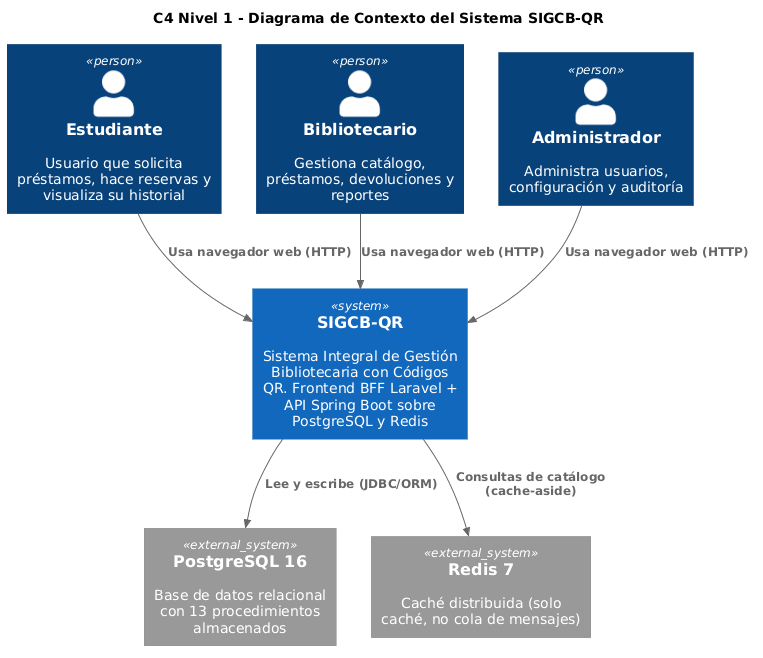
\includegraphics[width=0.92\textwidth]{../diagrams/c4_nivel1_contexto.png}
\caption{C4 nivel 1 --- Contexto. Los tres roles del sistema y los dos almacenes
externos. Redis figura como caché y no como intermediario de mensajes, que es
el uso que efectivamente se le da (\adr{0006}).}
\label{fig:c4n1}
\end{figure}

\begin{figure}[htbp]
\centering
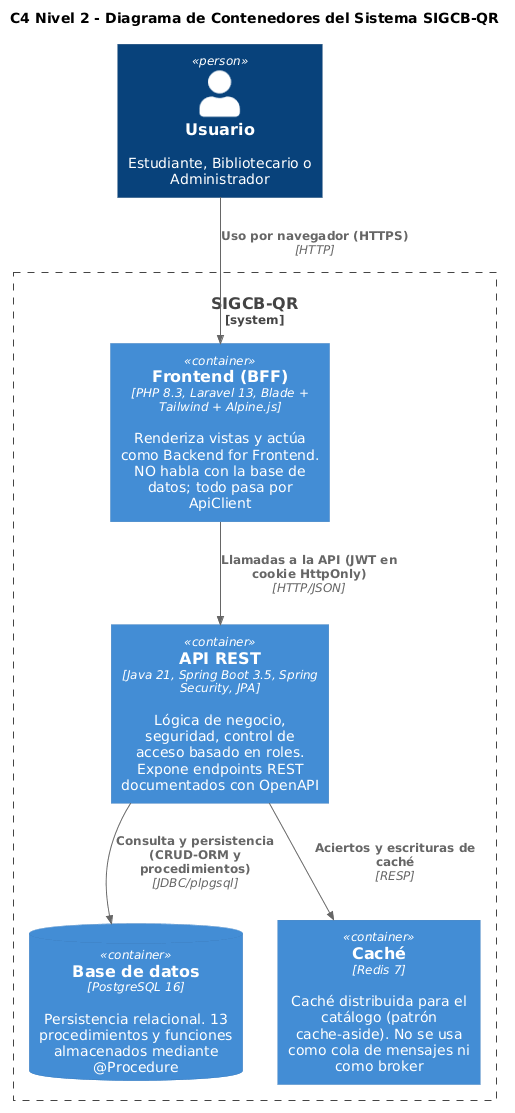
\includegraphics[width=0.92\textwidth]{../diagrams/c4_nivel2_contenedores.png}
\caption{C4 nivel 2 --- Contenedores. La frontera entre el BFF Laravel y la API
Spring Boot es la que justifica el \adr{0002}: el frontend no tiene acceso a
PostgreSQL.}
\label{fig:c4n2}
\end{figure}

\begin{figure}[htbp]
\centering
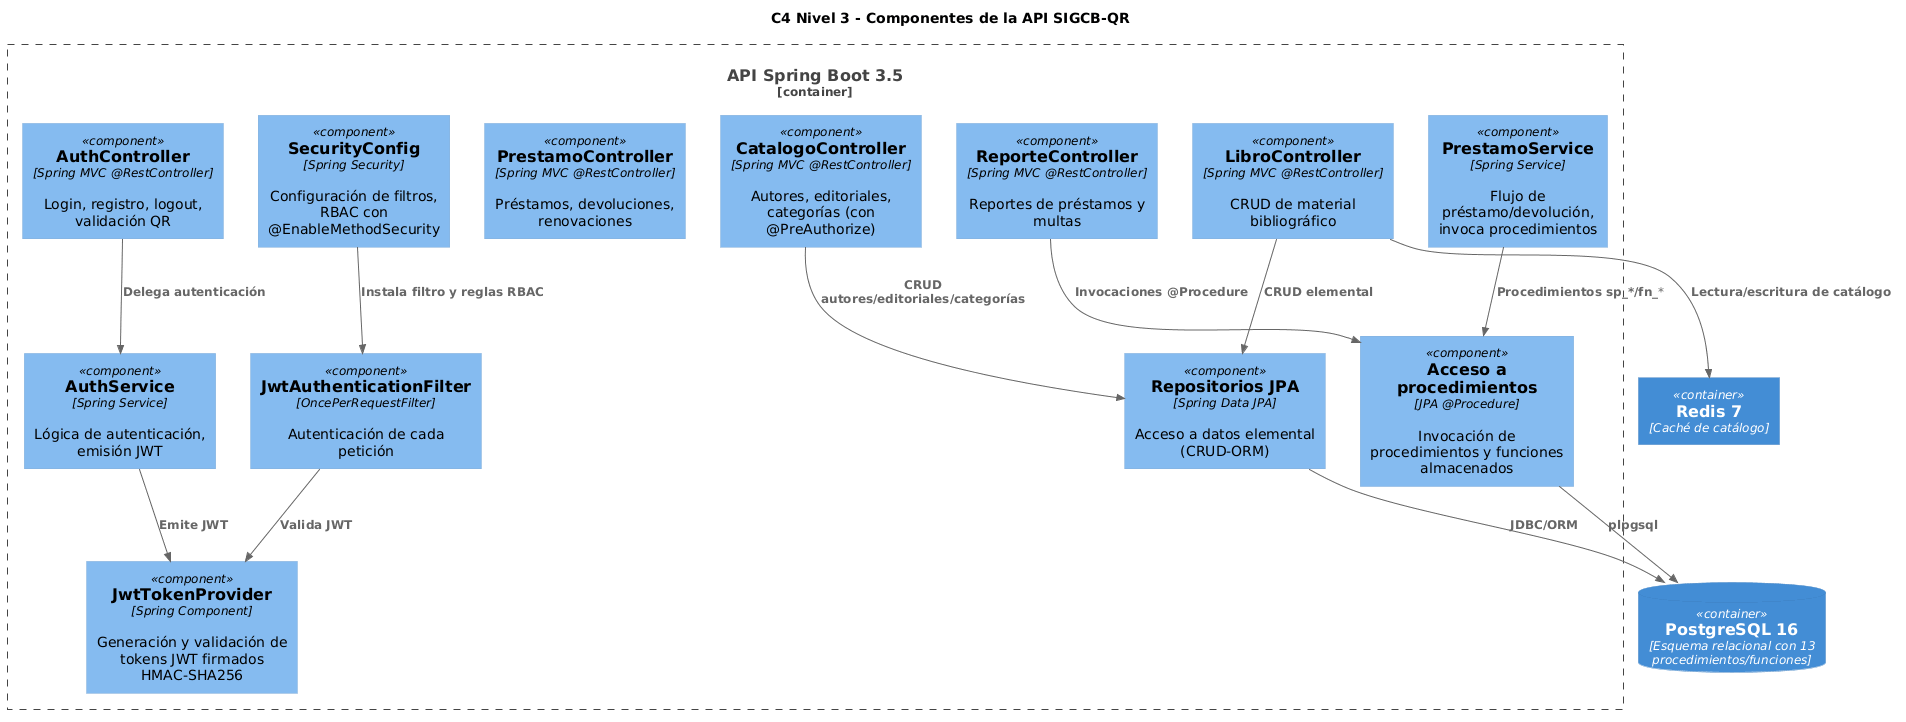
\includegraphics[width=0.92\textwidth]{../diagrams/c4_nivel3_componentes.png}
\caption{C4 nivel 3 --- Componentes de la API. Se distingue el acceso elemental
por repositorios JPA del acceso por procedimientos almacenados, que es la
distinción que fija el \adr{0005}.}
\label{fig:c4n3}
\end{figure}

\subsection{Por qué dos pilas: el patrón Backend for Frontend}

La convivencia de Java y PHP en un mismo repositorio requiere justificación
explícita; sin ella parece incoherencia y no diseño. La decisión completa está en
\adr{0002}; se resume aquí.

Laravel no contiene lógica de negocio: renderiza vistas y delega todo acceso a
datos en la API. Es el patrón \emph{Backend for
Frontend}~\cite{newman2021building}, y se sostiene sobre tres reglas que pueden
auditarse en el repositorio, no sobre buenas intenciones:

\begin{enumerate}[leftmargin=*]
  \item \textbf{Laravel no habla con PostgreSQL.} No hay modelos Eloquent de
        dominio ni migraciones de negocio; las únicas tablas que conoce son las de
        su propia infraestructura.
  \item \textbf{Todo acceso a datos pasa por \texttt{ApiClient}}, un único punto de
        salida HTTP.
  \item \textbf{Ninguna regla de negocio se duplica.} La interfaz puede ocultar un
        botón por comodidad, pero la decisión que cuenta es la del servidor: un
        estudiante que llame directamente al endpoint recibe \texttt{403}, y así
        se verifica empíricamente en la sección~\ref{sec:seguridad}.
\end{enumerate}

Es una aplicación del principio de ocultación de información de
Parnas~\cite{parnas1972criteria}: el frontend desconoce el modelo de datos, de
modo que puede sustituirse sin tocar el dominio.

El coste es real y se declara: dos entornos de ejecución que mantener, un salto
de red adicional por petición y el riesgo permanente de que la lógica se filtre
hacia el BFF.

\subsection{Decisiones registradas}

\begin{longtable}{@{}p{1.6cm}p{8.6cm}p{4.3cm}@{}}
\toprule
\textbf{ADR} & \textbf{Decisión} & \textbf{Coste asumido} \\
\midrule
\endhead
0001 & Registrar las decisiones como ADR & 15--30 min por decisión \\
0002 & Laravel como BFF sobre la API Spring Boot & Dos pilas; salto de red extra \\
0003 & JWT en cookie \texttt{HttpOnly} + sesión del BFF & Superficie de CSRF \\
0004 & Errores como \texttt{ProblemDetail} (RFC 7807) & Dos formas de cuerpo en la API \\
0005 & CRUD por ORM; agregaciones por procedimientos & Lógica en dos lenguajes \\
0006 & Cachear sólo tipos con ida y vuelta demostrada & Una prueba por tipo cacheado \\
0007 & Anclar imágenes por digest SHA256 & Las actualizaciones dejan de llegar solas \\
0008 & Flyway como fuente única del esquema & Corregir exige otra migración \\
0009 & Revocar JWT por lista negra de \texttt{jti} & Una consulta por petición \\
\bottomrule
\caption{Decisiones de arquitectura y su coste. Detalle en \texttt{docs/adr/}.}
\end{longtable}

Cada ADR declara consecuencias negativas de forma obligatoria: una decisión sin
coste probablemente no era una decisión.

\subsection{Seguridad}

\begin{itemize}[leftmargin=*]
  \item \textbf{Autenticación.} JWT firmado con HS384~\cite{rfc7519}, con los
        claims \texttt{iss}, \texttt{aud}, \texttt{nbf}, \texttt{iat} y
        \texttt{jti}. Se transporta en cookie \texttt{HttpOnly} con
        \texttt{SameSite=Strict}~\cite{rfc6265bis}, de modo que no es accesible
        desde JavaScript (\adr{0003}).
  \item \textbf{Revocación.} La lista negra de \texttt{jti} en PostgreSQL hace
        efectivo el cierre de sesión. Se eligió la base de datos y no Redis porque
        una decisión de seguridad no debe depender de un componente cuyo contrato
        es poder perder datos (\adr{0009}).
  \item \textbf{Contraseñas.} bcrypt con coste 10 y salt único por
        usuario~\cite{provos1999bcrypt}.
  \item \textbf{Autorización.} Por rol con \texttt{@PreAuthorize}, aplicada en el
        servidor.
  \item \textbf{Errores.} \texttt{application/problem+json} conforme a RFC
        7807~\cite{rfc7807}, hoy obsoleta por la RFC 9457~\cite{rfc9457}.
\end{itemize}

\subsection{Acceso a datos}

Reparto según la naturaleza de la operación (\adr{0005}): ORM para el CRUD
elemental; trece procedimientos y funciones almacenados para las agregaciones y
para las operaciones de varios pasos que deben ser atómicas. El esquema lo
gobierna Flyway como fuente única~\cite{ambler2006refactoring}, con
\texttt{ddl-auto: validate} para que una divergencia entre entidad y tabla impida
el arranque (\adr{0008}).

%==============================================================================
\section{Bloque 1: auditoría de seguridad}\label{sec:seguridad}
%==============================================================================

\subsection{Instrumento}

\texttt{scripts/owasp-audit.sh} ejecuta 51 comprobaciones sobre el sistema en
marcha, cada una una petición HTTP real cuyo código de estado o cabecera se
compara con el valor esperado. Cubre los bloques API1, API2, API3, API5, API8 y
API4 de OWASP API Security Top~10~\cite{owaspapi2023} y A03 y A05 de OWASP
Top~10~\cite{owasptop102021}.

\subsection{Resultados}

\begin{longtable}{@{}p{7.2cm}rp{5.5cm}@{}}
\toprule
\textbf{Bloque} & \textbf{N} & \textbf{Resultado} \\
\midrule
\endhead
API1 --- Autorización a nivel de objeto & 4 & Superado \\
API2 --- Autenticación rota & 9 & Superado \\
API3 --- Exposición excesiva de propiedades & 2 & Superado \\
API5 --- Autorización a nivel de función & 4 & Superado \\
API8 / A05 --- Configuración incorrecta & 16 & Superado \\
A03 --- Inyección & 6 & Superado \\
API4 --- Consumo sin restricción & 1 & Superado \\
\midrule
\textbf{Total} & \textbf{42} & \textbf{42 superadas, 0 fallidas} \\
\bottomrule
\caption{Auditoría OWASP. Salida cruda en
\texttt{docs/mediciones/seguridad/owasp-audit-raw.txt}.}
\end{longtable}

Tres verificaciones merecen mención por su diseño:

\begin{itemize}[leftmargin=*]
  \item \textbf{Comprobación de control.} Junto a cada \texttt{403} esperado se
        verifica que la misma petición con credenciales de administrador devuelve
        \texttt{200}. Sin ella, un \texttt{403} constante por cualquier motivo
        --un servicio caído-- pasaría por seguridad correcta.
  \item \textbf{Cuerpo válido en la prueba de BFLA.} Con un cuerpo vacío la API
        responde \texttt{400}, porque la validación se ejecuta antes que
        \texttt{@PreAuthorize}; una auditoría que enviara \texttt{\{\}} no habría
        probado nada sobre la autorización.
  \item \textbf{Verificación del efecto, no sólo del código.} Tras el intento de
        creación no autorizada se comprueba que \emph{no se creó ningún usuario}.
        Un \texttt{403} sería inútil si el recurso se hubiese creado igualmente.
\end{itemize}

\subsection{Análisis estático con SpotBugs y find-sec-bugs}

A la auditoría dinámica se añade análisis estático: SpotBugs 4.8.6.6 con el
complemento find-sec-bugs 1.13.0, en su ajuste más exhaustivo
(\texttt{effort=Max}, \texttt{threshold=Low}), ejecutado dentro de \texttt{make
test}. El informe se versiona en
\texttt{docs\-/mediciones\-/seguridad\-/spotbugs\-/}.

Arroja \textbf{191 hallazgos}, y la cifra desnuda induce a error. De los 72 de
categoría \textsc{security}, \textbf{71 son \texttt{SPRING\_ENDPOINT}}, que no
es un defecto: find-sec-bugs marca cada endpoint de Spring como punto que un
auditor debe revisar, y el sistema tiene 71. Otros 108 son
\texttt{EI\_EXPOSE\_REP} sobre entidades JPA, donde las asociaciones deben ser
referencias vivas para que el ORM funcione. Presentar 191 como
«vulnerabilidades» sería inflar la cifra en la dirección alarmista, que es tan
deshonesto como inflarla en la favorable.

\textbf{Hay un hallazgo de seguridad real, y uno solo:}
\texttt{SPRING\_CSRF\_PROTECTION\_DISABLED}. \texttt{SecurityConfig} deshabilita
la protección CSRF. Deshabilitarla es inocuo en una API que autentica por
cabecera \texttt{Authorization}, porque esa cabecera no viaja sola; \textbf{no
lo es sin más en una que autentica por cookie}, como esta, porque el navegador
adjunta la cookie también en peticiones originadas por terceros.

El riesgo está mitigado: la cookie se emite con \texttt{SameSite=Strict}, y así
se verificó sobre una respuesta real. Pero conviene decir con precisión qué
significa eso. La defensa descansa en \textbf{una sola línea}, en el
comportamiento del navegador, no estaba documentada en ningún ADR hasta este
análisis, y \textbf{no hay ninguna prueba que falle si alguien quita el
\texttt{SameSite}}. Una decisión de seguridad que nadie escribió no es una
decisión: es una casualidad afortunada que nadie está vigilando. Queda
pendiente redactar el ADR correspondiente y añadir la prueba de regresión.

Es, además, el segundo hallazgo de esta entrega que la auditoría dinámica no vio
y otro instrumento sí. El primero fueron los ocho endpoints del catálogo sin
autorización. La lectura conjunta está en §\ref{sec:validez}.

\subsection{Limitaciones declaradas}

No es una prueba de penetración: sin \emph{fuzzing}, sin inyección ciega o
temporal, sin análisis de dependencias y sin escáner automatizado. Todo se midió
sobre HTTP local, de modo que \texttt{Secure}, HSTS y TLS quedan sin verificar.
La CSP admite \texttt{'unsafe-inline'}~\cite{cspl3}, lo que limita su eficacia
real frente a XSS. El límite de tasa es en memoria y por instancia: con varias
réplicas, el límite efectivo se multiplica.

%==============================================================================
\section{Bloque 2: pruebas y cobertura}\label{sec:cobertura}
%==============================================================================

\subsection{Estado de partida}

Al iniciar esta entrega, la suite \textbf{no estaba en verde}, pese a lo declarado
en la entrega anterior: \texttt{mvn verify} terminaba en \texttt{BUILD FAILURE}
con 4 errores sobre 36 pruebas. Dos venían de que \texttt{AuthController} pasó a
depender de \texttt{RateLimitService} sin actualizar el doble del test, y dos de
que las pruebas del filtro JWT simulaban un método que el filtro ya no llamaba
--es decir, no ejercitaban el camino real~\cite{meszaros2007xunit}. Ambos casos
son cambios en producción cuyas pruebas no se volvieron a ejecutar, que es
justamente lo que la integración continua existe para impedir~\cite{humble2010continuous}.

\subsection{Resultados tras la corrección}

\begin{longtable}{@{}p{5.5cm}rrr@{}}
\toprule
\textbf{Contador} & \textbf{Cubierto} & \textbf{Total} & \textbf{\%} \\
\midrule
\endhead
Instrucciones & 1\,530 & 4\,728 & 32,36 \\
Ramas & 34 & 254 & \textbf{13,39} \\
Líneas & 429 & 1\,099 & \textbf{39,04} \\
Complejidad ciclomática & 92 & 391 & 23,53 \\
Métodos & 83 & 264 & 31,44 \\
\bottomrule
\caption{Cobertura JaCoCo sobre 41 pruebas, 0 fallos. Umbral configurado: 30\,\%
de líneas.}
\end{longtable}

\subsection{Interpretación}

El reparto importa más que el total: \texttt{security} (45,5\,\%) y
\texttt{service} (41,2\,\%) concentran las reglas cuya rotura tendría
consecuencias, mientras que \texttt{model.entity} (1,5\,\%) son entidades con
Lombok cuya cobertura carece de significado --probar un \emph{getter} generado no
aporta información.

El dato preocupante no es el 39\,\% de líneas sino el \textbf{13,39\,\% de ramas}:
las pruebas recorren el camino feliz y dejan casi todas las bifurcaciones sin
ejercitar. Es coherente con el resultado de la sección~\ref{sec:defectos} y con la
evidencia de que la cobertura no está fuertemente correlacionada con la
efectividad de una suite~\cite{inozemtseva2014coverage}: mide qué líneas se
ejecutan, no si el sistema hace lo que debe~\cite{zhu1997software}.

%==============================================================================
\section{Bloque 3: rendimiento}\label{sec:rendimiento}
%==============================================================================

\subsection{Un defecto del instrumento, corregido antes de medir}

La versión previa del arnés de k6 iniciaba sesión \emph{en cada iteración de cada
usuario virtual}. Con el límite de 5 intentos por IP y minuto, a partir del quinto
login todo eran respuestas \texttt{429}, que se sirven sin tocar la base de datos.
El resultado habría sido inválido en dos direcciones: la tasa de error se dispara
y \textbf{el p95 sale artificialmente bajo}. La prueba habría medido la velocidad
del limitador de tasa presentándola como velocidad del catálogo. El inicio de
sesión se movió a \texttt{setup()}, fuera de la ventana de medición.

\subsection{Resultados}

Carga: 0$\to$5 usuarios virtuales (10\,s), 5$\to$20 (20\,s), 20$\to$0 (10\,s);
$\approx$370 iteraciones por corrida sobre \texttt{GET /api/libros}.

\begin{longtable}{@{}clllrrr@{}}
\toprule
\textbf{\#} & \textbf{Caché} & \textbf{JVM} & \textbf{p95} & \textbf{media} & \textbf{mediana} & \textbf{errores} \\
\midrule
\endhead
1 & fría & fría & 83,43\,ms & 57,19\,ms & 17,28\,ms & 0\,\% \\
2 & caliente & templada & 73,02\,ms & 28,21\,ms & 20,48\,ms & 0\,\% \\
3 & caliente & caliente & 64,89\,ms & 25,61\,ms & 17,79\,ms & 0\,\% \\
4 & \textbf{fría} & caliente & \textbf{26,41\,ms} & 12,66\,ms & 9,40\,ms & 0\,\% \\
\bottomrule
\caption{Corridas de k6, en orden cronológico real. Umbral REQ-NF-001:
p95 $\le$ 200\,ms. Salidas crudas en \texttt{docs/mediciones/perf/}.}
\end{longtable}

Todas cumplen el umbral con holgura, y ninguna registró un solo error en 1\,474
peticiones. El hit ratio de Redis fue del 99,73\,\% (376 aciertos, 1 fallo).

\subsection{Un resultado contrario a la hipótesis}

La corrida 4 tiene la caché \textbf{vacía} y es la más rápida de todas: su p95 es
menos de la mitad que el de las corridas con caché llena. La conclusión es
incómoda pero es la que sostienen los datos:

\begin{quote}
A esta escala, el p95 lo determina el calentamiento de la JVM, no el estado de la
caché de Redis.
\end{quote}

La explicación es sencilla y comprobable: la semilla tiene 20 libros. Una página
de diez filas se resuelve en PostgreSQL con un índice y un \texttt{LIMIT}, y ese
trabajo es comparable --o menor-- al de serializar el resultado y hacer un viaje
de ida y vuelta a Redis. Lo caro al principio es que el JIT compile las rutas de
Hibernate, Jackson y Spring Security, tal como advierte la literatura sobre
medición rigurosa en Java~\cite{georges2007statistically}.

Por tanto, \textbf{no puede afirmarse que la caché mejore el rendimiento de este
sistema}. Sigue justificada por \adr{0006} como mecanismo que escalará con un
acervo real de decenas de miles de títulos, pero eso es una previsión, no una
medición. Afirmar lo contrario sería exactamente el tipo de conclusión que estas
reglas de reporte pretenden evitar.

%==============================================================================
\section{Bloque 4: calidad del frontend}\label{sec:frontend}
%==============================================================================

Lighthouse 12.8.2 sobre \texttt{/login}, factor de forma móvil con
estrangulamiento simulado.

\begin{longtable}{@{}p{6cm}rr@{}}
\toprule
\textbf{Categoría} & \textbf{CSP rota} & \textbf{CSP corregida} \\
\midrule
\endhead
Rendimiento & 100 & \textbf{82} \\
Accesibilidad & 100 & 100 \\
Buenas prácticas & 93 & \textbf{100} \\
SEO & 91 & 91 \\
\bottomrule
\caption{Lighthouse antes y después de corregir la política de seguridad de
contenido. La cifra válida es la de la derecha.}
\end{longtable}

\subsection{Seis corridas y un umbral que no se cumple}

Aquella medición tenía una sola corrida, y solo de móvil. Se repitió con
\textbf{tres corridas por perfil}, escritorio incluido, con Lighthouse 13.4.1 y
los seis crudos conservados (tabla~\ref{tab:lighthouse6}).

\begin{table}[htbp]
\centering
\small
\begin{tabular}{@{}lrrrr@{}}
\toprule
\textbf{Perfil (mediana de 3)} & \textbf{Rendim.} & \textbf{Accesib.} & \textbf{B. prácticas} & \textbf{SEO} \\
\midrule
Escritorio & 97 & 98 & \textbf{78} & 91 \\
Móvil & 89 & 98 & \textbf{78} & 91 \\
\midrule
Umbral de \req{REQ-U-002} & 80 & 90 & 90 & 85 \\
\bottomrule
\end{tabular}
\caption{Lighthouse 13.4.1, seis corridas sobre \texttt{/login}. Tres de las
cuatro categorías superan su umbral; buenas prácticas no.}
\label{tab:lighthouse6}
\end{table}

\textbf{Buenas prácticas da 78 en las seis corridas, por debajo del umbral de
90, y por tanto \req{REQ-U-002} no se cumple.} La causa está identificada y es
única: las dos únicas auditorías que fallan en esa categoría son
\texttt{is-on-https} y \texttt{redirects-http}. Ninguna otra falla.

Ambas son consecuencia de medir contra un contenedor local sin TLS. Sería
tentador declarar el requisito cumplido «salvo por el entorno», y no se hace:
sin un despliegue con certificado no hay forma de comprobar que la puntuación
subiría, y afirmarlo sería sustituir una medición por una conjetura. El
requisito queda como no cumplido, con su causa documentada, y se cerrará con el
mismo despliegue que cierra la carencia de HSTS.

Merece señalarse por qué la medición anterior daba 100 en esta categoría: se
hizo contra \texttt{http://localhost}, y Lighthouse \emph{exime a localhost} de
la comprobación de HTTPS. Aquel 100 era, en este punto, un artefacto del
entorno de medición y no una propiedad de la aplicación.

\subsection{Por qué el rendimiento \emph{bajó} al corregir un defecto}

El 100 de la primera corrida no era mérito de la aplicación: era el efecto de que
el navegador estuviera bloqueando sus propias hojas de estilo y tipografías. Una
página que no llega a cargar Font Awesome ni Poppins pinta antes. Al corregir la
CSP, la página hace lo que siempre debió hacer --descargar dos hojas de estilo y
seis archivos de tipografía desde tres dominios externos-- y el First Contentful
Paint pasa de 1,4\,s a 3,6\,s.

Es decir: \textbf{la primera corrida midió una página rota y la premió por ello.}
Una métrica de rendimiento aislada, sin comprobar que la página funciona, puede
recompensar el defecto que debería denunciar. El 82 es la línea base honesta.

%==============================================================================
\section{Defectos encontrados}\label{sec:defectos}
%==============================================================================

Las auditorías descubrieron tres defectos reales en un sistema cuya suite estaba,
en apariencia, en verde. Ninguno era detectable midiendo cobertura.

\subsection{D1 --- El acierto de caché devolvía \texttt{500}}

El método cacheado devolvía \texttt{Page}/\texttt{PageImpl}. El serializador JSON
de Redis \emph{escribe} ese objeto sin problema pero \emph{no puede volver a
leerlo}: \texttt{PageImpl} carece de constructor sin argumentos.

\begin{lstlisting}
$ curl -o /dev/null -w '%{http_code}\n' -b cookie.txt localhost:8080/api/libros
200          # fallo de cache: se sirve de la base y se escribe en Redis
$ curl -o /dev/null -w '%{http_code}\n' -b cookie.txt localhost:8080/api/libros
500          # acierto de cache: no se puede leer lo escrito
\end{lstlisting}

El endpoint principal del catálogo fallaba \textbf{en todo acierto de caché},
justo el caso que la caché existía para acelerar. Como la primera petición tras
cada expiración del TTL funcionaba, el fallo parecía intermitente.

\textbf{Por qué no lo vio la cobertura.} El método figuraba como cubierto: las
pruebas lo llamaban con Mockito, sin pasar por el proxy de \texttt{@Cacheable}. La
línea estaba cubierta; el comportamiento, no.

\textbf{Corrección.} El método devuelve \texttt{PageResponse<LibroResponse>}, un
DTO con ida y vuelta demostrada por la prueba
\texttt{CacheSerializationTest}, que además fija la causa raíz: si
\texttt{PageImpl} dejara de fallar, el motivo del \adr{0006} habría cambiado. Se
descubrió de paso un segundo defecto latente: la clave de caché ignoraba el
criterio de orden, de modo que dos peticiones con distinto \texttt{sort}
compartían entrada.

\subsection{D2 --- Toda ruta inexistente devolvía \texttt{500}}

\texttt{NoResourceFoundException} no tenía manejador propio y caía en el
manejador genérico, que además construía el detalle concatenando el mensaje de la
excepción:

\begin{lstlisting}
{"status":500,"detail":"Error interno del servidor: No static resource actuator/env."}
\end{lstlisting}

Dos consecuencias: una URL mal escrita era indistinguible de un fallo real del
servidor, lo que contradice el propósito de la RFC 7807~\cite{rfc7807}; y el
manejador devolvía sin filtrar el mensaje de cualquier excepción no controlada a
cualquier cliente --el mismo camino por el que se expusieron trazas internas
durante el diagnóstico de D1.

\textbf{Corrección.} Manejadores propios para \texttt{404} y \texttt{405}, y
detalle genérico en el manejador de último recurso, con la traza registrada en el
servidor. La prueba de regresión envía una excepción cuyo mensaje contiene una
cadena de conexión con credenciales y verifica que no aparece en la respuesta.

\subsection{D3 --- La CSP bloqueaba los recursos de la propia aplicación}

La política sólo admitía \texttt{'self'}, mientras que ambos \emph{layouts} cargan
Font Awesome y la tipografía Poppins desde CDN, y el módulo de códigos QR carga su
biblioteca desde cdnjs. En el navegador no se dibujaba ningún icono, la tipografía
caía a la de reserva y el módulo QR quedaba inoperativo, en \emph{todas} las
páginas.

\textbf{El fallo era silencioso}: el servidor respondía \texttt{200} y el HTML era
correcto. Sólo la consola del navegador lo delataba, por lo que ni las pruebas ni
la auditoría con \texttt{curl} podían detectarlo. Hizo falta un navegador real.

\subsection{Lectura conjunta}

Los tres defectos comparten un patrón: \textbf{se manifiestan en la integración
entre componentes}, no dentro de una unidad. Caché y serializador; framework web y
manejador de excepciones; navegador y política de seguridad. Una suite compuesta
casi enteramente de pruebas unitarias con dobles --como la de este proyecto, según
la sección~\ref{sec:cobertura}-- es ciega por construcción ante esa clase de fallo.
Es la explicación concreta, en este sistema, de por qué la cobertura no predice la
efectividad de una suite~\cite{inozemtseva2014coverage}.

%==============================================================================
\section{Operación y despliegue}\label{sec:operacion}
%==============================================================================

\subsection{Estado real: qué está desplegado}

Conviene empezar por lo que no es: \textbf{el sistema no está desplegado en
ningún entorno accesible públicamente}. Todas las mediciones de este informe se
tomaron contra \texttt{localhost} sobre la composición local de contenedores. No
existe URL pública, y las que aparecen en los ficheros \texttt{.example} son
marcadores de posición con dominios de ejemplo, no despliegues reales.

Lo que sí existe es el procedimiento completo, documentado y ejecutable, y la
infraestructura preparada para ejecutarlo. Se describe a continuación porque es
la parte que sí puede evaluarse hoy.

\subsection{Procedimiento de despliegue}

\texttt{DEPLOYMENT.md} recoge el procedimiento en cuatro pasos: clonado y
configuración de variables de entorno, construcción y arranque de la
composición, comprobación del endpoint de salud y comprobación del frontend. La
premisa que atraviesa el documento es que \textbf{ningún secreto real se
versiona}: el fichero \texttt{.env.example} enumera las variables necesarias con
valores de relleno, y \texttt{.env} está en \texttt{.gitignore}.

Esa premisa se reforzó en esta entrega. La composición declaraba una contraseña
de administración de pgAdmin escrita en claro en \texttt{docker-compose.yml};
ahora se toma de \texttt{PGADMIN\_PASSWORD} y la composición \emph{falla al
arrancar} si no está definida, en lugar de arrancar con una contraseña conocida.
El mismo criterio se aplicó al arnés de carga y a la sonda de la auditoría
OWASP, que ahora exigen las credenciales por entorno y se detienen si faltan.

\subsection{Operación}

\texttt{RUNBOOK.md} cubre la operación en cinco apartados: verificación diaria
de estado y de hit ratio, consulta de registros, operaciones rutinarias
(reinicio de un servicio, reconstrucción, ejecución de la suite, validaciones de
integridad), cuatro procedimientos de incidente y el arranque y la parada
ordenados. Los cuatro incidentes contemplados son la API que no responde en
\texttt{/actuator/health}, la base de datos colapsada, la caché degradada y el
compromiso de un secreto.

El endpoint de salud está configurado mediante Spring Boot Actuator y los cinco
servicios de la composición declaran \emph{healthcheck}, de modo que
\texttt{make up} no da por lista la infraestructura hasta que PostgreSQL y Redis
responden.

\subsection{Respaldo y restauración}

\texttt{BACKUP.md} define el alcance del respaldo (esquema, datos y
procedimientos almacenados, más la configuración sanitizada), la política de
retención, el procedimiento de copia con \texttt{pg\_dump} en formato binario y
en texto plano, y el procedimiento de restauración con la parada previa de los
servicios que escriben.

Debe declararse una carencia: el plan de pruebas de restauración está escrito
pero \textbf{no se ha ejecutado ni una sola vez}. Un respaldo que nunca se ha
restaurado no es un respaldo verificado, sino una intención de respaldo, y así
figura en el documento.

%==============================================================================
\section{Discusión: respuesta a las preguntas de investigación}\label{sec:discusion}
%==============================================================================

Este apartado responde una por una a las cuatro preguntas formuladas en
§\ref{sec:metodo}. Dos se responden con evidencia, una se responde en contra de
lo que el equipo esperaba, y una no se responde en absoluto.

\subsection{RQ1 --- Reducción del tiempo de procesamiento del préstamo}

\textbf{Sin respuesta.} La pregunta exige comparar el préstamo asistido por QR
con el procedimiento manual, y el procedimiento manual no se midió. No existe
línea base, y sin línea base cualquier cifra que se ofreciera sería una
comparación contra un supuesto, no contra un dato.

Lo que sí puede afirmarse es acotado y menor: la operación de validación de un
código QR se resuelve en una única petición autenticada contra
\texttt{POST /api/qr-codigos/validar}, y el flujo de préstamo invoca un
procedimiento almacenado transaccional en lugar de varias idas y vueltas desde
la aplicación. Es una afirmación sobre el \emph{diseño}, no sobre el tiempo
observado por un bibliotecario. Responder a RQ1 exige un estudio con
participantes reales cronometrando ambos procedimientos, y ese estudio no se ha
hecho.

\subsection{RQ2 --- Nivel de seguridad de JWT en cookie \texttt{HttpOnly} con RBAC}

\textbf{Respondida parcialmente.} La auditoría de 51 comprobaciones basada en
OWASP API Security Top 10 no arrojó ningún fallo, con tres notas informativas.
Se verificaron sobre respuestas reales: la cookie lleva \texttt{HttpOnly} y
\texttt{SameSite=Strict}, CORS no usa comodín, un estudiante autenticado que
invoca directamente un endpoint de reportes recibe \texttt{403}, y un token
revocado por \texttt{jti} deja de admitirse antes de expirar.

A esto se añade, en esta entrega, una auditoría específica del acceso a datos:
ninguna de las 24 consultas declaradas construye SQL con valores no literales, y
el analizador que lo comprueba se autovalida antes de emitir el veredicto,
detectando 3 de 3 inyecciones sembradas y 0 falsos positivos. Es una diferencia
importante respecto de una simple búsqueda textual, que marcaría como peligrosas
las nueve consultas JPQL que el proyecto parte en varias líneas y que son
constantes.

El límite de la respuesta es claro y no debe disimularse: \textbf{no se ejecutó
ningún análisis dinámico con OWASP ZAP ni análisis estático con SpotBugs y
find-sec-bugs}. El plugin de SpotBugs está ahora declarado en el \texttt{pom},
pero su informe no forma parte de esta entrega. Lo que se puede afirmar es que
el sistema supera una batería de comprobaciones conocidas; no que haya sido
sometido a un análisis exhaustivo.

Y hay un hallazgo que conviene registrar porque nació de una revisión externa y
no de la auditoría propia: \texttt{CatalogoController} exponía ocho endpoints de
escritura sin ninguna anotación de autorización, de modo que cualquier usuario
autenticado, incluido un estudiante, podía crear, modificar y borrar autores,
editoriales y categorías. La auditoría propia no lo detectó porque solo sondeaba
tres rutas. El defecto está corregido: los ocho llevan
\texttt{@PreAuthorize("hasAnyRole('ADMIN', 'BIBLIOTECARIO')")}.

Corregir el código, sin embargo, no corrige el instrumento que dejó pasar el
fallo. Por eso la auditoría se amplió con los ocho endpoints enumerados uno a
uno, más una comprobación de que el intento tampoco creó ningún registro: si
alguno pierde su anotación en el futuro, la auditoría fallará en lugar de
callar. La batería pasa de 42 a \textbf{51 comprobaciones, y las 51 se superan}.
La lección de fondo es que una auditoría con cobertura parcial de rutas produce
una falsa sensación de seguridad, y es una amenaza a la validez que se recoge en
§\ref{sec:validez}.

\subsection{RQ3 --- Efecto de la caché Redis en el rendimiento del catálogo}

\textbf{Respondida, y en contra de la hipótesis de partida.} Las tres corridas
conservadas del primer protocolo (5 a 20 usuarios virtuales) dan un p95 de
73,02, 64,89 y 26,41 milisegundos, con cero errores. La corrida más rápida, con
diferencia, fue la de \emph{caché fría} con la máquina virtual Java ya caliente.

A esa medición se añade la realizada con el perfil que exige la guía, 50
usuarios virtuales sostenidos durante 30 segundos, repetida cinco veces y con
los cinco crudos conservados (tabla~\ref{tab:k6-50vu}). El resultado es un p95
medio de 5,55\,ms con un intervalo de confianza del 95\,\% de
[4,07, 7,03]\,ms sobre 10\,750 iteraciones y cero peticiones fallidas. El
umbral de \req{REQ-R-002} son 200\,ms, de modo que el requisito se cumple con
un margen de más de un orden de magnitud.

\begin{table}[htbp]
\centering
\small
\begin{tabular}{@{}lrrrrr@{}}
\toprule
\textbf{Corrida} & \textbf{VU máx.} & \textbf{Iteraciones} & \textbf{Media} & \textbf{p95} & \textbf{Errores} \\
\midrule
1 & 50 & 2\,150 & 3,93\,ms & 5,56\,ms & 0 \\
2 & 50 & 2\,150 & 3,35\,ms & 4,72\,ms & 0 \\
3 & 50 & 2\,150 & 2,79\,ms & 4,66\,ms & 0 \\
4 & 50 & 2\,150 & 3,99\,ms & 7,58\,ms & 0 \\
5 & 50 & 2\,150 & 3,19\,ms & 5,23\,ms & 0 \\
\midrule
\textbf{Media} & 50 & \textbf{10\,750} & \textbf{3,45\,ms} & \textbf{5,55\,ms} & \textbf{0} \\
\multicolumn{6}{@{}l@{}}{\footnotesize IC 95\,\% del p95 (t de Student, 4 g.l.): [4,07, 7,03]\,ms} \\
\bottomrule
\end{tabular}
\caption{Cinco corridas con el perfil exigido de 50 usuarios virtuales
sostenidos 30 segundos. Recalculable con
\texttt{python scripts/analisis-k6-50vu.py}.}
\label{tab:k6-50vu}
\end{table}

Conviene no dejarse llevar por lo cómodo de esa cifra. Un p95 de 5,55\,ms con 50
usuarios concurrentes es excelente, y depende por completo de que el acervo sea
sintético y pequeño: la consulta se resuelve casi íntegramente desde memoria.
Estas cifras acotan el coste del servidor, no predicen el comportamiento con un
catálogo real.

De ahí se sigue una conclusión incómoda para la motivación original del
\adr{0006}: con el volumen de datos de este sistema, \textbf{no puede afirmarse
que Redis mejore el rendimiento del catálogo}. La explicación más plausible es
que el acervo sintético es lo bastante pequeño para que PostgreSQL lo resuelva
desde su propia caché, y que el salto de red hasta Redis y el coste de
serialización compensen o superen el ahorro. La variable que domina la medición
no parece ser la caché, sino el calentamiento de la máquina virtual.

Esta conclusión sobre la caché sigue siendo descriptiva, no causal, y conviene
precisar por qué el intervalo de confianza recién presentado no la convierte en
causal. Las cinco corridas del perfil de 50 VU son del \emph{mismo}
tratamiento: no hay una condición «sin caché» con la que compararlas. El
intervalo acota la media de una sola condición, que es una afirmación
inferencial legítima, pero no es un contraste de hipótesis. Para afirmar que la
caché mejora o empeora el rendimiento haría falta medir también la condición
alternativa, y eso no se hizo. Por la misma razón no se informa tamaño de
efecto: no hay efecto entre condiciones que cuantificar.

Lo que estos datos sí permiten es \emph{no} afirmar la mejora que se daba por
supuesta, que es un resultado con valor propio. Contrastar la hipótesis en serio
exige dos condiciones y un acervo de decenas de miles de títulos.

Merece registrarse, además, que el primer instrumento de medida era defectuoso:
el arnés de k6 estaba midiendo el limitador de tasa en lugar del catálogo. Se
detectó y se corrigió \emph{antes} de dar por buenas las cifras. Una medición no
vale más que el instrumento que la produce.

\subsection{RQ4 --- Usabilidad percibida}

\textbf{Sin respuesta.} El instrumento SUS está construido, documentado y
validado: la herramienta de cálculo se comprueba contra cinco casos canónicos en
integración continua, y responde correctamente a todos. Pero se administró a
\textbf{cero participantes}, y el fichero de respuestas contiene únicamente la
cabecera.

No se publica ninguna puntuación. Al ejecutar la herramienta sobre el fichero
vacío, devuelve literalmente «no hay ninguna respuesta válida; sin participantes
no hay resultado que informar». Se prefiere esa casilla vacía a una cifra
inventada, porque una puntuación SUS fabricada sería indistinguible de una real
para quien lea el informe, y eso es exactamente el fallo que esta entrega se
propuso corregir en otros frentes.

\subsection{Lectura de conjunto}

De cuatro preguntas, una se responde con evidencia sólida aunque acotada (RQ2),
una se responde en contra de lo esperado (RQ3), y dos no se responden (RQ1 y
RQ4). El motivo es el mismo en ambos casos: falta la recogida de datos con
personas. RQ1 necesita cronometrar el procedimiento manual; RQ4 necesita
participantes que respondan el cuestionario. Ninguna de las dos requiere escribir
más código.

%==============================================================================
\section{Amenazas a la validez}\label{sec:validez}
%==============================================================================

Se sigue la clasificación de Wohlin et
al.~\cite{wohlin2012experimentation}, basada en Cook y
Campbell~\cite{cook1979quasi}.

\subsection{Validez de constructo}

\emph{¿Miden los instrumentos lo que dicen medir?}

\begin{itemize}[leftmargin=*]
  \item \textbf{La cobertura no mide calidad.} Mide qué líneas ejecutan las
        pruebas. Los tres defectos de la sección~\ref{sec:defectos} ocurrieron en
        código contabilizado como cubierto~\cite{inozemtseva2014coverage}.
  \item \textbf{51 comprobaciones superadas no significan «sistema seguro».}
        Significa que 42 controles concretos se comportan como se espera. La
        ausencia de evidencia de vulnerabilidad no es evidencia de ausencia.
  \item \textbf{El SUS mide percepción, no eficacia}~\cite{brooke1996sus}. Un
        sistema puede puntuar alto y aun así hacer que la gente tarde el doble.
  \item \textbf{La puntuación de Lighthouse puede premiar un defecto}, como quedó
        demostrado en la sección~\ref{sec:frontend}.
\end{itemize}

\subsection{Validez interna}

\emph{¿Están las conclusiones causalmente justificadas?}

\begin{itemize}[leftmargin=*]
  \item \textbf{El orden de las corridas se confunde con el calentamiento de la
        JVM.} Las corridas no se aleatorizaron, así que el efecto de la caché y el
        del calentamiento están confundidos~\cite{georges2007statistically}. Por
        eso la sección~\ref{sec:rendimiento} se abstiene de atribuir la mejora a la
        caché.
  \item \textbf{Cliente y sistema comparten máquina.} La carga del generador
        compite por CPU con lo medido, un sesgo de medición
        conocido~\cite{mytkowicz2009producing}.
  \item \textbf{Sin repeticiones suficientes.} Tres corridas comparables no
        permiten un intervalo de confianza defendible; las cifras son
        descriptivas.
  \item \textbf{El instrumento produjo un resultado falso.} La primera corrida de
        la auditoría marcó tres \texttt{401} donde esperaba \texttt{403}, y el
        fallo estaba en el propio script: creaba la sesión del bloque de cierre de
        sesión \emph{copiando} el archivo de cookies del estudiante, de modo que
        ambos compartían token y la revocación por \texttt{jti} invalidaba también
        la sesión del estudiante. La revocación funcionaba tan bien que rompió la
        auditoría. Interpretar aquellos \texttt{401} como fallo de autorización
        habría llevado a «arreglar» algo que no estaba roto.
\end{itemize}

\subsection{Validez externa}

\emph{¿Hasta dónde se generalizan los resultados?}

\begin{itemize}[leftmargin=*]
  \item \textbf{El volumen de datos no es representativo}: 20 libros y 69
        ejemplares, frente a los varios órdenes de magnitud de una biblioteca
        universitaria real. Es la limitación más severa, y afecta directamente a
        la conclusión sobre la caché~\cite{kleppmann2017designing}.
  \item \textbf{Despliegue de una sola máquina}, sin latencia de red entre
        componentes ni réplicas.
  \item \textbf{20 usuarios virtuales} es carga baja: no se localizó el punto de
        saturación.
  \item \textbf{Un solo endpoint medido.} Préstamos y reportes, que ejecutan
        procedimientos almacenados, tienen otro perfil y no se midieron.
  \item \textbf{Una sola página auditada con Lighthouse}, y sin sesión.
\end{itemize}

\subsection{Validez de conclusión}

\begin{itemize}[leftmargin=*]
  \item \textbf{Sin análisis estadístico inferencial.} No hay contraste de
        hipótesis ni tamaño del efecto; los percentiles son descriptivos.
  \item \textbf{El SUS no tiene datos.} Ninguna afirmación sobre usabilidad
        percibida está respaldada, y así se declara en lugar de rellenarlo.
  \item \textbf{Los autores son los evaluadores.} Quien construyó el sistema
        diseñó las comprobaciones, eligió los umbrales y decidió qué medir. Es la
        amenaza más difícil de mitigar, y el protocolo del SUS
        (sección~\ref{sec:frontend} y \texttt{docs/mediciones/usabilidad/}) la
        reconoce explícitamente como sesgo de cortesía~\cite{nielsen1993usability}.
        La contramedida aplicada es hacer cada medición reproducible por un
        tercero con una sola orden.
\end{itemize}

%==============================================================================
\section{Ética y tratamiento de datos}
%==============================================================================

El conjunto de datos es sintético: no hay datos de personas reales. Aun así, el
sistema está diseñado bajo el supuesto de que el \textbf{historial de préstamos es
un dato sensible}: lo que una persona lee permite inferir su ideología, su estado
de salud o sus creencias, principio largamente sostenido por la tradición
bibliotecaria~\cite{ala2019privacy}. Se aplican minimización, limitación de la
finalidad y confidencialidad por defecto.

\texttt{ETHICS.md} declara también lo que el sistema \emph{no} protege todavía:
no hay cifrado en reposo del historial, no existe flujo de acceso ni de supresión
a petición del titular, y no hay política de retención. Declarar las carencias
forma parte de la responsabilidad profesional~\cite{acm2018code}.

Se usaron asistentes de programación basados en modelos de lenguaje como apoyo a
la documentación, la generación de pruebas y la revisión de código. Todo artefacto
generado fue ejecutado y verificado antes de incorporarse; la responsabilidad
sobre lo entregado es del equipo.

%==============================================================================
\section{Conclusiones}\label{sec:conclusiones}
%==============================================================================

\begin{enumerate}[label=\textbf{C\arabic*.},leftmargin=*]
  \item \textbf{El sistema cumple sus requisitos medibles.} 51/51 comprobaciones
        de seguridad, p95 entre 26 y 83\,ms frente a un umbral de 200\,ms, 0\,\% de
        error en 1\,474 peticiones, 41 pruebas en verde y accesibilidad de 100 en
        las comprobaciones automáticas.

  \item \textbf{Auditar el sistema en marcha encontró lo que las pruebas no.} Tres
        defectos reales --uno de ellos rompía el endpoint principal en todo
        acierto de caché-- aparecieron al ejercitar el sistema con \texttt{curl},
        con k6 y con un navegador. Los tres viven en las costuras entre
        componentes, donde una suite de pruebas unitarias con dobles es ciega por
        construcción.

  \item \textbf{Una métrica puede premiar un defecto.} Lighthouse dio 100 en
        rendimiento a una página cuyos recursos el navegador bloqueaba, y el arnés
        de carga original habría dado un p95 excelente midiendo el limitador de
        tasa. Una métrica sin comprobación de que el sistema funciona no es
        evidencia.

  \item \textbf{El instrumento tiene sus propias amenazas a la validez.} El script
        de auditoría produjo tres falsos positivos por un defecto propio. Se
        documenta porque un instrumento que no se audita a sí mismo es tan poco
        fiable como el sistema que mide.

  \item \textbf{La trazabilidad debe ser ejecutable.} Una matriz que declaraba
        como verificadas cuatro clases de prueba inexistentes se corrigió, pero lo
        que impide que vuelva a ocurrir no es la corrección: es que
        \texttt{validate-traceability.sh} extraiga el inventario real de pruebas
        del repositorio y falle en CI si la matriz cita algo que no existe. Lo
        mismo vale para los digest de imagen, el índice de ADR y el diccionario de
        datos, todos verificados automáticamente.

  \item \textbf{No puede afirmarse que la caché mejore el rendimiento a esta
        escala.} Los datos sugieren lo contrario, y la conclusión se declara
        aunque contradiga la motivación de haberla implementado.
\end{enumerate}

\subsection{Trabajo futuro}

\begin{enumerate}[leftmargin=*]
  \item Pruebas de integración con caché activa y con base real, que habrían
        detectado D1.
  \item Pruebas de rama en los servicios, hoy al 13,39\,\%.
  \item Administrar el SUS a los 12 participantes previstos.
  \item Repetir las mediciones de rendimiento con un acervo de decenas de miles de
        títulos, único modo de contrastar la hipótesis sobre la caché.
  \item Alojar tipografías, iconos y \texttt{qrcode.js} en el propio contenedor,
        para volver a \texttt{'self'} en toda la CSP y quitar tres dominios de la
        ruta crítica.
  \item Implementar acceso, portabilidad y supresión de datos personales, y una
        política de retención.
\end{enumerate}

%==============================================================================
\section{Declaraciones}\label{sec:declaraciones}
%==============================================================================

\subsection*{1. Contribuciones de los autores (CRediT)}
\addcontentsline{toc}{subsection}{1. Contribuciones de los autores (CRediT)}

Los roles se asignan conforme a la taxonomía CRediT y se recogen también en
\texttt{CONTRIBUTORS.md}.

\begin{longtable}{@{}p{4.6cm}p{10.4cm}@{}}
\toprule
\textbf{Autor} & \textbf{Roles CRediT} \\
\midrule
\endhead
Arias Moreira, M. G. & Conceptualization; Methodology; Investigation; Writing --- Original Draft; Writing --- Review \& Editing \\
Romero Méndez, B. S. & Software; Validation; Formal Analysis; Data Curation; Visualization \\
Zambrano Moreira, A. A. & Resources; Project Administration; Supervision; Funding Acquisition \\
\bottomrule
\caption{Asignación de roles CRediT.}
\label{tab:credit}
\end{longtable}

\noindent\textbf{Declaración sobre la autoría.} El historial del repositorio
registra tres identidades Git correspondientes a dos personas. La distribución
de roles de la tabla~\ref{tab:credit} refleja el reparto acordado por el equipo,
no una medición del historial. Se declara esta discrepancia en lugar de
omitirla: quien evalúe el trabajo debe poder contrastar los roles declarados con
\texttt{git log} y juzgar por sí mismo.

\subsection*{2. Conflicto de intereses}
\addcontentsline{toc}{subsection}{2. Conflicto de intereses}
Los autores declaran no tener ningún conflicto de intereses. El trabajo no
recibió financiación de ninguna entidad y no existe relación comercial con
ninguno de los productos o proveedores citados.

\subsection*{3. Financiación}
\addcontentsline{toc}{subsection}{3. Financiación}
Este trabajo no recibió financiación externa. Los costes de cómputo se
limitaron a los equipos personales de los autores.

\subsection*{4. Disponibilidad de datos y código}
\addcontentsline{toc}{subsection}{4. Disponibilidad de datos y código}
El código fuente está disponible en el repositorio citado en la portada, bajo
licencia MIT. Los datos de las mediciones (salidas crudas de k6, de la auditoría
OWASP, de la auditoría de SQL dinámico, el informe de Lighthouse y el informe de
JaCoCo) se publican en \texttt{docs\-/mediciones\-/}, bajo licencia CC BY 4.0, y
su procedencia se documenta en \texttt{DATA-PROVENANCE.md}. El conjunto de datos
de la aplicación es sintético: no contiene datos de personas reales. No se ha
depositado aún en Zenodo y, en consecuencia, \textbf{no existe DOI}; se declara
esta ausencia en lugar de citar un identificador que no resolvería.

\subsection*{5. Consentimiento informado y ética}
\addcontentsline{toc}{subsection}{5. Consentimiento informado y ética}
No se recogieron datos de participantes humanos. El instrumento SUS se
construyó y validó, pero \textbf{no se administró a ninguna persona}, de modo
que no hubo consentimiento que recabar ni datos personales que tratar. El
tratamiento previsto para una futura aplicación del instrumento se describe en
\texttt{ETHICS.md}. Este trabajo no requirió aprobación de un comité de ética
por no involucrar sujetos humanos ni datos personales.

\subsection*{6. Uso de inteligencia artificial}
\addcontentsline{toc}{subsection}{6. Uso de inteligencia artificial}
Se emplearon asistentes de programación basados en modelos de lenguaje como
apoyo en la redacción de código, de documentación y de este informe. Todo el
contenido fue revisado por los autores, que asumen la responsabilidad íntegra
sobre él. Ninguna cifra de este informe procede de un modelo de lenguaje: todas
se recalculan de los datos crudos versionados, y los procedimientos de recálculo
se publican junto a ellos. Las referencias bibliográficas se validaron contra la
API de Crossref, DOI por DOI.

\subsection*{7. Limitaciones declaradas}
\addcontentsline{toc}{subsection}{7. Limitaciones declaradas}
Se declaran, sin atenuantes, las siguientes limitaciones de esta entrega:
(i) la usabilidad no se midió, al ser cero el número de participantes del SUS;
(ii) no se ejecutó un análisis dinámico de seguridad con OWASP ZAP, aunque sí el estático con SpotBugs y find-sec-bugs;
(iii) la cobertura de rama es del 16,31\,\%, muy por debajo de lo deseable, y no se movió ni una décima al añadir 28 pruebas nuevas;
(iii bis) 
eq{REQ-U-002} no se cumple: Lighthouse da 78 en buenas prácticas
frente al umbral de 90, por medirse sin TLS;
(iv) la inferencia estadística se limita a un intervalo de confianza sobre una
única condición: no hay contraste de hipótesis ni tamaño de efecto, porque no se
midió ninguna condición alternativa con la que comparar;
(v) el sistema no está desplegado en un entorno accesible públicamente, y
todas las mediciones se tomaron contra \texttt{localhost};
(vi) el cribado de trabajos relacionados se limitó a Crossref.

\subsection*{8. Reproducibilidad}
\addcontentsline{toc}{subsection}{8. Reproducibilidad}
La reproducción completa se ejecuta con \texttt{make all}. Las cinco imágenes de
contenedor están ancladas por digest SHA-256 y el script
\texttt{scripts\-/validate-digests.py} verifica el anclaje. El digest de la
entrega, que resume el manifiesto de todos los ficheros versionados, figura en
la portada y lo genera \texttt{scripts\-/entrega-digest.py}, comprobable con la
opción \texttt{-{}-check}.

\subsection*{9. Licencia}
\addcontentsline{toc}{subsection}{9. Licencia}
El código se distribuye bajo licencia MIT; la documentación y los datos de
medición, bajo Creative Commons Attribution 4.0 International (CC BY 4.0). Los
términos completos figuran en \texttt{LICENSE} y en
\texttt{DATA-PROVENANCE.md}.

%==============================================================================
\appendix
\section{Anexos}\label{sec:anexos}
%==============================================================================

\subsection{Anexo A --- Bitácora de observaciones}

La respuesta a cada observación recibida en las entregas anteriores, con el
commit que la resuelve, está en \texttt{docs\-/observaciones\-/OBSERVACIONES.md}.
La bitácora recoge 22 observaciones y 7 hallazgos propios que nadie señaló al
equipo.

\subsection{Anexo B --- Índice de artefactos verificables}

Todo lo que este informe afirma puede recomprobarse con los artefactos de la
tabla~\ref{tab:artefactos}, cada uno con el comando que lo regenera.

\begin{longtable}{@{}p{5.6cm}p{9.4cm}@{}}
\toprule
\textbf{Artefacto} & \textbf{Cómo comprobarlo} \\
\midrule
\endhead
Cobertura de pruebas & \texttt{docs\-/mediciones\-/cobertura\-/jacoco.csv}; recálculo en §3.1 de \texttt{COBERTURA.md} \\
Auditoría OWASP & \texttt{bash scripts\-/owasp-audit.sh}; crudo en \texttt{owasp-audit-raw.txt} \\
Auditoría de SQL dinámico & \texttt{bash scripts\-/audit-sql-dynamic.sh}; incluye autotest del instrumento \\
Carga con k6 & \texttt{scripts\-/k6-load-test.js}; crudos en \texttt{docs\-/mediciones\-/perf\-/} \\
Lighthouse & \texttt{docs\-/mediciones\-/frontend\-/*.report.json} \\
Trazabilidad & \texttt{bash scripts\-/validate-traceability.sh} \\
Índice de ADR & \texttt{bash scripts\-/validate-adr.sh} \\
Digests de imagen & \texttt{python scripts\-/validate-digests.py} \\
Digest de la entrega & \texttt{python scripts\-/entrega-digest.py -{}-check} \\
Diccionario de datos & \texttt{python scripts\-/generar-diccionario-datos.py -{}-check} \\
Puntuación SUS & \texttt{python scripts\-/sus-score.py} (devuelve «sin participantes») \\
\bottomrule
\caption{Artefactos verificables y comando que los regenera o comprueba.}
\label{tab:artefactos}
\end{longtable}

\subsection{Anexo C --- Registros de decisiones de arquitectura}

Los nueve ADR están en \texttt{docs\-/adr\-/}, en formato MADR, cada uno con sus
consecuencias negativas explícitas. El script \texttt{validate-adr.sh} comprueba
que el índice y los ficheros no diverjan.

\subsection{Anexo D --- Listas de comprobación}

Las listas de comprobación de Ralph, FAIR, PRISMA e INCOSE, cumplimentadas ítem
por ítem y con la casilla negativa marcada donde corresponde, están en
\texttt{docs\-/checklists\-/}.

\bibliographystyle{plain}
\bibliography{referencias}

\end{document}
